\documentclass{standalone}
\usepackage{tikz}
\usetikzlibrary{patterns, positioning}


\begin{document}
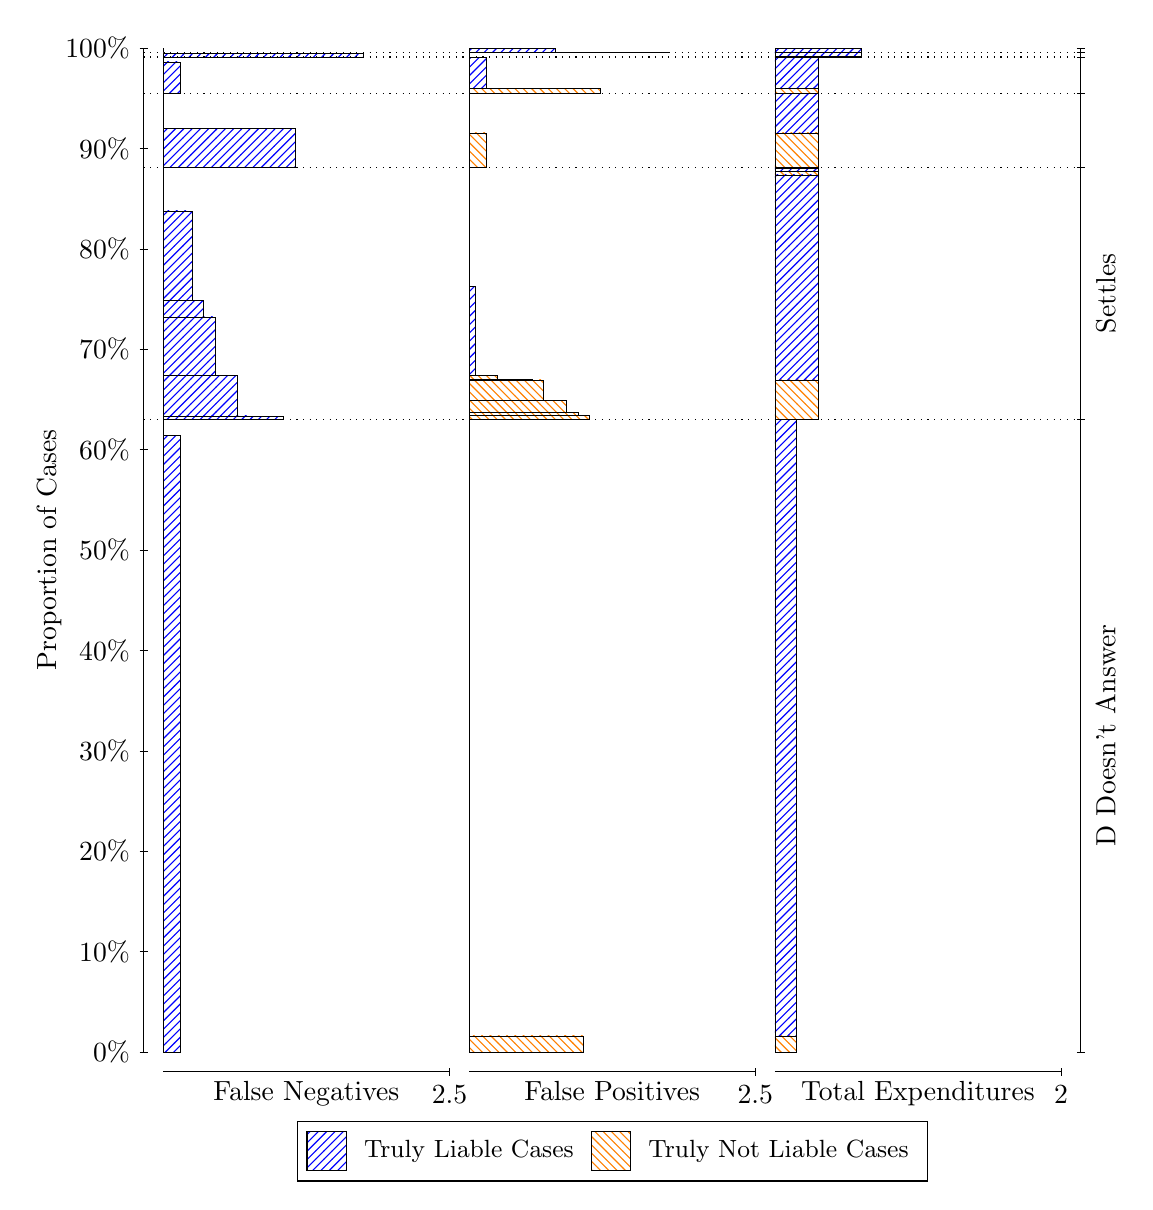
\begin{tikzpicture}
\draw[black, very thin] (1.5,1.75) -- (1.5,14.5);
\node[rotate=90, text=black, anchor=center] at (0.3, 8.125) {Proportion of Cases};
\draw[black, very thin] (1.45,1.75) -- (1.55,1.75);
\node[text=black, anchor=east] at (1.45, 1.75) {0\%};
\draw[black, very thin] (1.45,3.025) -- (1.55,3.025);
\node[text=black, anchor=east] at (1.45, 3.025) {10\%};
\draw[black, very thin] (1.45,4.3) -- (1.55,4.3);
\node[text=black, anchor=east] at (1.45, 4.3) {20\%};
\draw[black, very thin] (1.45,5.575) -- (1.55,5.575);
\node[text=black, anchor=east] at (1.45, 5.575) {30\%};
\draw[black, very thin] (1.45,6.85) -- (1.55,6.85);
\node[text=black, anchor=east] at (1.45, 6.85) {40\%};
\draw[black, very thin] (1.45,8.125) -- (1.55,8.125);
\node[text=black, anchor=east] at (1.45, 8.125) {50\%};
\draw[black, very thin] (1.45,9.4) -- (1.55,9.4);
\node[text=black, anchor=east] at (1.45, 9.4) {60\%};
\draw[black, very thin] (1.45,10.675) -- (1.55,10.675);
\node[text=black, anchor=east] at (1.45, 10.675) {70\%};
\draw[black, very thin] (1.45,11.95) -- (1.55,11.95);
\node[text=black, anchor=east] at (1.45, 11.95) {80\%};
\draw[black, very thin] (1.45,13.225) -- (1.55,13.225);
\node[text=black, anchor=east] at (1.45, 13.225) {90\%};
\draw[black, very thin] (1.45,14.5) -- (1.55,14.5);
\node[text=black, anchor=east] at (1.45, 14.5) {100\%};

\draw[black, very thin] (13.4,1.75) -- (13.4,14.5);
\draw[black, very thin] (13.35,1.75) -- (13.45,1.75);
\node[anchor=west] at (13.35, 1.75) {};
\draw[black, very thin] (13.35,9.788) -- (13.45,9.788);
\node[anchor=west] at (13.35, 9.788) {};
\draw[black, very thin] (13.35,12.981) -- (13.45,12.981);
\node[anchor=west] at (13.35, 12.981) {};
\draw[black, very thin] (13.35,13.925) -- (13.45,13.925);
\node[anchor=west] at (13.35, 13.925) {};
\draw[black, very thin] (13.35,14.386) -- (13.45,14.386);
\node[anchor=west] at (13.35, 14.386) {};
\draw[black, very thin] (13.35,14.44) -- (13.45,14.44);
\node[anchor=west] at (13.35, 14.44) {};
\draw[black, very thin] (13.35,14.5) -- (13.45,14.5);
\node[anchor=west] at (13.35, 14.5) {};

\draw[black, very thin, pattern color=blue, pattern=north east lines] (1.75,1.75) rectangle (1.968,9.5838);
\draw[black, very thin, pattern color=orange, pattern=north west lines] (1.75,9.5838) rectangle (1.75,9.788);
\draw[black, very thin, pattern color=blue, pattern=north east lines] (1.75,9.788) rectangle (3.276,9.8252);
\draw[black, very thin, pattern color=blue, pattern=north east lines] (1.75,9.8252) rectangle (2.84,9.828);
\draw[black, very thin, pattern color=blue, pattern=north east lines] (1.75,9.828) rectangle (2.6947,10.347);
\draw[black, very thin, pattern color=blue, pattern=north east lines] (1.75,10.347) rectangle (2.404,11.085);
\draw[black, very thin, pattern color=blue, pattern=north east lines] (1.75,11.085) rectangle (2.2587,11.295);
\draw[black, very thin, pattern color=blue, pattern=north east lines] (1.75,11.295) rectangle (2.1133,12.431);
\draw[black, very thin, pattern color=orange, pattern=north west lines] (1.75,12.431) rectangle (1.75,12.981);
\draw[black, very thin, pattern color=blue, pattern=north east lines] (1.75,12.981) rectangle (3.4213,13.483);
\draw[black, very thin, pattern color=orange, pattern=north west lines] (1.75,13.483) rectangle (1.75,13.925);
\draw[black, very thin, pattern color=blue, pattern=north east lines] (1.75,13.925) rectangle (1.968,14.324);
\draw[black, very thin, pattern color=orange, pattern=north west lines] (1.75,14.324) rectangle (1.75,14.386);
\draw[black, very thin, pattern color=blue, pattern=north east lines] (1.75,14.386) rectangle (4.2933,14.428);
\draw[black, very thin, pattern color=orange, pattern=north west lines] (1.75,14.428) rectangle (1.75,14.44);
\draw[black, very thin, pattern color=orange, pattern=north west lines] (1.75,14.44) rectangle (1.75,14.445);
\draw[black, very thin, pattern color=blue, pattern=north east lines] (1.75,14.445) rectangle (1.75,14.5);
\draw[black, very thin, pattern color=orange, pattern=north west lines] (5.6333,1.75) rectangle (7.0867,1.9541);
\draw[black, very thin, pattern color=blue, pattern=north east lines] (5.6333,1.9541) rectangle (5.6333,9.788);
\draw[black, very thin, pattern color=orange, pattern=north west lines] (5.6333,9.788) rectangle (7.1593,9.8333);
\draw[black, very thin, pattern color=orange, pattern=north west lines] (5.6333,9.8333) rectangle (7.014,9.8721);
\draw[black, very thin, pattern color=orange, pattern=north west lines] (5.6333,9.8721) rectangle (6.8687,10.025);
\draw[black, very thin, pattern color=orange, pattern=north west lines] (5.6333,10.025) rectangle (6.578,10.286);
\draw[black, very thin, pattern color=orange, pattern=north west lines] (5.6333,10.286) rectangle (6.4327,10.289);
\draw[black, very thin, pattern color=orange, pattern=north west lines] (5.6333,10.289) rectangle (5.9967,10.338);
\draw[black, very thin, pattern color=blue, pattern=north east lines] (5.6333,10.338) rectangle (5.706,11.474);
\draw[black, very thin, pattern color=blue, pattern=north east lines] (5.6333,11.474) rectangle (5.6333,12.981);
\draw[black, very thin, pattern color=orange, pattern=north west lines] (5.6333,12.981) rectangle (5.8513,13.423);
\draw[black, very thin, pattern color=blue, pattern=north east lines] (5.6333,13.423) rectangle (5.6333,13.925);
\draw[black, very thin, pattern color=orange, pattern=north west lines] (5.6333,13.925) rectangle (7.3047,13.987);
\draw[black, very thin, pattern color=blue, pattern=north east lines] (5.6333,13.987) rectangle (5.8513,14.386);
\draw[black, very thin, pattern color=orange, pattern=north west lines] (5.6333,14.386) rectangle (5.6333,14.398);
\draw[black, very thin, pattern color=blue, pattern=north east lines] (5.6333,14.398) rectangle (5.6333,14.44);
\draw[black, very thin, pattern color=orange, pattern=north west lines] (5.6333,14.44) rectangle (8.1767,14.445);
\draw[black, very thin, pattern color=blue, pattern=north east lines] (5.6333,14.445) rectangle (6.7233,14.5);
\draw[black, very thin, pattern color=orange, pattern=north west lines] (9.5167,1.75) rectangle (9.7892,1.9541);
\draw[black, very thin, pattern color=blue, pattern=north east lines] (9.5167,1.9541) rectangle (9.7892,9.788);
\draw[black, very thin, pattern color=orange, pattern=north west lines] (9.5167,9.788) rectangle (10.062,10.286);
\draw[black, very thin, pattern color=blue, pattern=north east lines] (9.5167,10.286) rectangle (10.062,12.889);
\draw[black, very thin, pattern color=orange, pattern=north west lines] (9.5167,12.889) rectangle (10.062,12.938);
\draw[black, very thin, pattern color=blue, pattern=north east lines] (9.5167,12.938) rectangle (10.062,12.975);
\draw[black, very thin, pattern color=orange, pattern=north west lines] (9.5167,12.975) rectangle (10.062,12.978);
\draw[black, very thin, pattern color=blue, pattern=north east lines] (9.5167,12.978) rectangle (10.062,12.981);
\draw[black, very thin, pattern color=orange, pattern=north west lines] (9.5167,12.981) rectangle (10.062,13.423);
\draw[black, very thin, pattern color=blue, pattern=north east lines] (9.5167,13.423) rectangle (10.062,13.925);
\draw[black, very thin, pattern color=orange, pattern=north west lines] (9.5167,13.925) rectangle (10.062,13.987);
\draw[black, very thin, pattern color=blue, pattern=north east lines] (9.5167,13.987) rectangle (10.062,14.386);
\draw[black, very thin, pattern color=orange, pattern=north west lines] (9.5167,14.386) rectangle (10.607,14.398);
\draw[black, very thin, pattern color=blue, pattern=north east lines] (9.5167,14.398) rectangle (10.607,14.44);
\draw[black, very thin, pattern color=orange, pattern=north west lines] (9.5167,14.44) rectangle (10.607,14.445);
\draw[black, very thin, pattern color=blue, pattern=north east lines] (9.5167,14.445) rectangle (10.607,14.5);
\draw[black, dotted] (1.5,9.788) -- (13.4,9.788);
\draw[black, dotted] (1.5,12.981) -- (13.4,12.981);
\draw[black, dotted] (1.5,13.925) -- (13.4,13.925);
\draw[black, dotted] (1.5,14.386) -- (13.4,14.386);
\draw[black, dotted] (1.5,14.44) -- (13.4,14.44);
\draw[black, very thin] (1.75,1.5) -- (5.3833,1.5);
\node[text=black, anchor=north] at (3.5667, 1.5) {False Negatives};
\draw[black, very thin] (5.3833,1.45) -- (5.3833,1.55);
\node[text=black, anchor=north] at (5.3833, 1.45) {2.5};

\draw[black, very thin] (5.6333,1.5) -- (9.2667,1.5);
\node[text=black, anchor=north] at (7.45, 1.5) {False Positives};
\draw[black, very thin] (9.2667,1.45) -- (9.2667,1.55);
\node[text=black, anchor=north] at (9.2667, 1.45) {2.5};

\draw[black, very thin] (9.5167,1.5) -- (13.15,1.5);
\node[text=black, anchor=north] at (11.333, 1.5) {Total Expenditures};
\draw[black, very thin] (13.15,1.45) -- (13.15,1.55);
\node[text=black, anchor=north] at (13.15, 1.45) {2};

\node[text=black, centered, rotate=90] at (13.72, 5.769) {D Doesn't Answer};
\node[text=black, centered, rotate=90] at (13.72, 11.385) {Settles};





\draw (7.449999999999999,1.5) node[draw=none] (baseCoordinate) {};
\begin{scope}[align=center]
        \matrix[scale=0.5, draw=black, below=0.5cm of baseCoordinate, nodes={draw}, column sep=0.1cm]{
            \node[rectangle, draw, minimum width=0.5cm, minimum height=0.5cm, pattern color=blue, pattern=north east lines] {}; &
            \node[draw=none, font=\small, text=black] (B) {Truly Liable Cases}; &
            \node[rectangle, draw, minimum width=0.5cm, minimum height=0.5cm, pattern color=orange, pattern=north west lines] {}; &
            \node[draw=none, font=\small, text=black] (B) {Truly Not Liable Cases}; \\
            };
\end{scope}

\end{tikzpicture}
\end{document}